\chapter{Question3}
\section{问题概述}
%
%%对问题的直观描述
%
本问题要求利用神经网络进行数字分类。

%
%对项目已有代码的阅读和理解
%

%
%解决问题的思路和想法
%

\section{算法设计}
%
%用自己的语言描述解决问题所使用的算法的原理及功能,设计思路和算法流程图
%
所用的神经网络架构与上一题一样,唯一的区别在于特征向量维数从1变为了$28\times28$,输出向量维数由1变为了10,同时判断训练是否结束
的依据变为了由在验证集上得到的准确率。
\section{算法实现}
%
%在算法原理的基础上,结合代码,讲述算法的实现细节、核心函数、模块输入输出,数据结构定义等内容
%
%
\begin{lstlisting}[emph={[3]dataset,x,y},emphstyle={[3]\color{vscode_parametercolor}},emph={[4]DigitClassificationModel,RegressionModel,GameState,MinimaxAgent,AlphaBetaAgent},emphstyle={[4]\color{vscode_classcolor}}]
class DigitClassificationModel(object):
    def __init__(self):
        self.layer_size = 512
        self.feature_num = 28*28
        self.output_num = 10
        self.learning_rate = 0.5
        self.batch_size = 200
        self.threshold = 0.98
        self.w1 = nn.Parameter(self.feature_num,self.layer_size)
        self.b1 = nn.Parameter(1,self.layer_size)
        self.w2 = nn.Parameter(self.layer_size,self.output_num)
        self.b2 = nn.Parameter(1,self.output_num)
        self.W = [self.w1,self.b1,self.w2,self.b2]

    def run(self, x):
        return nn.AddBias( nn.Linear( nn.ReLU( nn.AddBias( nn.Linear(x,self.w1),self.b1)),self.w2),self.b2)

    def get_loss(self, x, y):
        return nn.SoftmaxLoss(self.run(x),y)

    def train(self, dataset):
        for x,y in dataset.iterate_forever(self.batch_size):
            gradients = nn.gradients(self.get_loss(x,y),self.W)
            for i,w in enumerate(self.W):
                w.update(gradients[i],-self.learning_rate)
            if dataset.get_validation_accuracy() >= self.threshold:
                break
\end{lstlisting}
\section{实验结果}
我成功获得了本问题的所有分数。本问的评分依据便是训练好的神经网络在测试集上得到的准确率。
\begin{figure}[htbp]
    \centering
    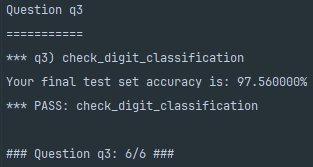
\includegraphics{pic/q3.png}
    \caption{Question3实验结果}\label{q3}
\end{figure}
%
%实验中遇到的问题及解决方案,收获和思考:对算法的理解、优缺点的评价、算法的适用场景
%
